\documentclass{article}
\usepackage{iclr2027_conference,times}
\usepackage{amsmath,amssymb,booktabs,graphicx,microtype}
\usepackage{pifont}
\usepackage[colorlinks=true,linkcolor=blue,citecolor=blue]{hyperref}
% cleveref unavailable in this TeX install; \ref used directly

\title{Conditional Nulls and Positive Controls for Task-Vector Subspace Overlap}
\author{Anonymous}

\begin{document}
\maketitle
\begin{abstract}
Task-vector subspace overlap is often interpreted as shared learned structure because it exceeds
an isotropic baseline, although linear-layer updates depend on the activations they read. We
introduce a conditional randomisation that preserves each update's spectrum and blockwise
occupancy in frozen-base activation geometry while randomising cross-task directional agreement;
its expected overlap has a closed form. We pair this null with a positive control that plants
shared directions and measures recovery of the delivered signal, exposing consequential
under-randomisation in our initial implementation. In complete ViT-B measurements, the corrected
activation null reproduces about a quarter of above-isotropic overlap, moving over $20$--$26\%$
across our calibration and blocking grid at the reported subspace size, and the residual stays
positive throughout. Module role moves this far
more than architecture does. For shared-start LoRA a regime-matched factor null reproduces about
$80\%$, but a one-line count from the shared rank already gives $82\%$, so there the admissible
row space, not a learned basis, accounts for nearly all observed overlap. These are attribution
statements conditional on what each null holds fixed, and they leave pair rankings and downstream
merge behaviour unchanged.
\end{abstract}

\section{Introduction}

Independently fine-tuned models built on one pre-trained checkpoint have task vectors whose
input-side singular subspaces overlap far above an isotropic random baseline, and a growing body
of merging work measures that overlap and builds on it.
\citet{gargiulo2025task} report the cross-task inner products of right singular vectors and
define an interference score from them.
\citet{demystify2026} define a Right Subspace Overlap statistic over $190$ pairs of task vectors
and use it as one input to a predictor of merging success.
\citet{qiu2026nufilt} construct a null-space projector out of the cumulative update's right
singular vectors, and justify it with a theorem that task vectors approximately align with
representation subspaces.
In each case the overlap is compared, explicitly or implicitly, against what an unstructured
subspace would give.

That comparison is correct for unconditional random subspaces, but it does not answer the
conditional attribution question studied here. For a linear map $y=Wh$, the raw minibatch
gradient has the outer-product form
\begin{equation}
 \nabla_W L_t=\sum_{b\in\mathcal B_t}g_{t,b}h_{t,b}^\top.
 \label{eq:outer-product}
\end{equation}
Under scalar-step gradient descent without weight decay, the final update's row space therefore
lies in the span of the activations along that specialist's own training trajectory. This exact statement neither
identifies a common frozen-base span nor applies unchanged after coordinatewise optimiser
preconditioning: activations drift and optimisers transform gradients. It motivates a weaker,
measurable question. Using the frozen base's activation second moment as a common coordinate
system, how much observed overlap is predicted after holding fixed each update's own occupancy
of that geometry? The isotropic value $k/d_{\mathrm{in}}$ conditions on none of it.

Prior work motivates both sides of this question. \citet{cheng2025wudi} relate linear-layer task
vectors to their inputs, and \citet{qiu2026nufilt} give an approximate subspace-alignment result;
the latter note that the effect of shared initialisation remains insufficiently explored. These
results do not establish frozen-base containment for the checkpoints studied here. Cross-task
right-subspace overlap itself is already measured at scale by the work above. What is missing is
a stated conditional baseline, an accounting of how much the answer moves under it, and evidence
that the baseline randomises what it claims to.

We provide all three. The activation-conditioned null independently acts on each observed update
with rotations that preserve its complete singular spectrum and blockwise read-mass profile in
the frozen-base activation eigenbasis. Its expectation has a closed form: it is the overlap
predicted by the two observed occupancy profiles. The remainder is residual directional
agreement conditional on them. This is an operational conditional decomposition; the retained
profile is measured after fine-tuning and may itself contain task-learned structure. A generative
alternative sampled from $C_H$ is not a valid conditional comparator because it must invent the
update--activation relationship and produces a conspicuous level failure in our
common-reference stress test.

Applied to the CLIP benchmarks used by this literature, the null reproduces $25.3\%$ and $22.4\%$
of above-isotropic top-$8$ overlap in the two complete ViT-B measurements. Conditional on the
fixed calibration and blocking specification, the remaining excess stays positive throughout the
crossed task--layer finite-pool stability interval. Under rank-$16$
LoRA, $\mathrm{row}(BA)\subseteq\mathrm{row}(A)$ makes the observed $A$ factor a necessary
regime-specific condition. Its top-$8$ right singular subspaces overlap at $0.88$, and at $1.00$
when linearisation keeps $A$ bit-identical, while the learned $B$ factor's top-$8$ left singular
subspaces overlap at $0.05$ against $0.01$ isotropic
chance. An $A$- and factor-spectrum-conditioned null reproduces $80.3\%$ of the product update's
above-isotropic overlap;
although its attainable plant delivers only $37.4$--$57.0\%$ of the nominal increment, the null
recovers $100.7$--$101.1\%$ of what is delivered. This one stress test does not identify which
mechanism produced the conditioned structure.

The methodological result is why these estimates, rather than a larger number from our first
implementation, are reported. A zero-signal level check accepts the identity map, so it cannot
detect under-randomisation. We add a positive control that plants shared directions and measures
the signal actually delivered and recovered. It exposed two under-randomisation defects in the
activation null and a nuisance-spectrum mismatch in the LoRA null. Correcting the activation
null raised delivered-signal recovery from $45.6$--$51.7\%$ to $99.3$--$99.6\%$ and moved the full-
fine-tuning ViT-B/16 headline from roughly $67\%$ to $25.3\%$. Surrogates independently drawn from that conditional
null also form a relative stress test: the isotropic and participation-ratio-whitened baselines
report $+0.0171$ and $+0.0522$ apparent excess. This comparison is conditional on our stated
reference model and is not an independent intervention.

We make three contributions: a group-conditional decomposition of read-subspace overlap; a
positive-control protocol that checks power as well as level and catches consequential defects in
our own nulls; and a regime-specific audit of full fine-tuning and LoRA that separates effect-size
attribution from pair ranking and downstream merge performance.

\section{Related work}
\label{sec:related}

\paragraph{Subspace overlap in model merging.}
Merging grew from weight averaging~\citep{wortsman2022soups,ilharco2022patching,matena2022fisher}
through task arithmetic~\citep{ilharco2023editing,ortizjimenez2023tangent} to interference
resolved coordinate by coordinate~\citep{yadav2023ties,yu2024dare} and then in
subspaces~\citep{stoica2025knots,tang2023concrete,lee2025star}, which is where overlap became a
reported quantity.
\citet{cheng2025wudi} relate linear-layer task vectors to their corresponding inputs and
\citet{qiu2026nufilt} give an approximate subspace-alignment result. These works motivate
activation-aware conditioning; they do not imply exact containment in a frozen-base subspace
under feature drift and adaptive optimisation. The overlap measurement is established by
\citet{gargiulo2025task}, \citet{demystify2026} and \citet{marczak2025iso}, none of which states a
conditional reference distribution for it. Our contribution is that conditional baseline and a
protocol for checking how much coupling it actually randomises.

\paragraph{Activation statistics as machinery.}
Activation second moments are long-standing, and continual learning has used them longest.
\citet{saha2021gpm} build gradient subspace bases by SVD of stored input activations and
\citet{wang2021nullspace} project updates into the null space of the uncentered input feature
covariance, the same object as our $C_H$. Both use it to constrain training.
Inside merging the pattern repeats: RegMean~\citep{jin2023dataless} merges with per-model input
Gram matrices computed on each fine-tuned model's own data, and two data-free methods estimate
the covariance from the parameter differences~\citep{actmat2026,acemerging2026}.
More directly, \citet{an2025pave} compute pre-linear-layer covariances from each task's training
examples and fine-tuned model to construct a knowledge-aware SVD for pruning task vectors.
All target a task-conditioned object, $\mathbb{E}_{x \sim \mathcal{D}_t}[xx^\top]$. We instead
choose the frozen base under a recorded calibration mixture as a common, task-agnostic coordinate
system; this is part of our estimand rather than a uniquely necessary null.
Using $\Delta W^\top\Delta W$ itself as a reference would also be circular: exact inverse-square-root
whitening equalises the nonzero singular values and makes a top-$k$ choice non-identifiable rather
than supplying an independent calibration geometry. What none supplies is a statement of what an uninformative task vector looks like, and the
difference bites: RegMean's published shrinkage returns $2.3\times$ chance on independent task
vectors when repurposed as an evidential baseline
(Appendix~\ref{app:calibration}).

\paragraph{Null models for similarity claims.}
\citet{cui2022deconfounded} show that representation-similarity metrics such as RSA and
CKA~\citep{kornblith2019similarity,raghu2017svcca} are confounded by the population structure
of the input data, giving ``spuriously high similarity for
even completely random neural networks''.
Our conditional analysis is the weight-space analogue: there the shared object is population
structure in the input distribution, while here the conditioned object is occupancy of a common
activation geometry and the measured quantity is task-vector subspace overlap.
\citet{ding2021grounding} make the complementary point for the measures themselves, arguing
that a similarity metric must be judged on sensitivity to changes that matter and specificity
against changes that do not, which is the pairing \S\ref{sec:validate} imports for nulls.
The general form is older. \citet{elsayed2017structure} formalise whether population-level
structure exceeds what already-known primary features predict, by comparing against surrogate
data that preserves those features and is otherwise maximally random.
The null of \S\ref{sec:method} is that construction applied to weights, and \S\ref{sec:validate}
is the part of the surrogate-data tradition this literature has not imported: checking what the
surrogate actually destroys.

\paragraph{Low-rank adapters.}
How a shared adapter basis should be read is what \S\ref{sec:exp} bears on, and several
methods construct or exploit one~\citep{stoica2025knots,panariello2025corespace,zeng2026tvbases}.
The geometric result has a functional counterpart already known.
\citet{zhu2024asymmetry} show that in $\Delta W = BA$ the two factors are not interchangeable:
fine-tuning $B$ is substantially more effective than fine-tuning $A$, and a random untrained $A$
performs nearly as well as a trained one.
If $A$ need not be trained to work, it is unsurprising that it carries little task-specific
information.
\citet{ban2026rethinking} reach the qualitative conclusion directly, reporting that the
similarity between $A$ matrices across adapters is attributable to the identical
initialisation and not to shared knowledge. That conclusion is theirs.
We add the geometric constraint, $\mathrm{row}(\Delta W) \subseteq \mathrm{row}(A)$, and a
factor-conditioned null whose reproduced fraction we report with its measured response and scope.

\section{A null for task-vector subspace overlap}
\label{sec:method}

\subsection{What is being measured, and against what}

For a pair of task vectors $\Delta W_i, \Delta W_j \in \mathbb{R}^{d_{\mathrm{out}} \times d_{\mathrm{in}}}$
let $V_i^{(k)}$ hold the top-$k$ right singular vectors of $\Delta W_i$, and write
\begin{equation}
\mathcal{O}(i,j) \;=\; \tfrac{1}{k}\,\big\|\, V_i^{(k)\top} V_j^{(k)} \,\big\|_F^2 ,
\label{eq:overlap}
\end{equation}
the mean squared canonical correlation between the two read subspaces.
For two independent uniformly random $k$-subspaces of $\mathbb{R}^{d_{\mathrm{in}}}$ this has
expectation $k/d_{\mathrm{in}}$, which we verify numerically in
Appendix~\ref{app:invariants}; that value is the isotropic null the literature reports against.

The question is not whether $\mathcal{O}$ exceeds $k/d_{\mathrm{in}}$. It does, by an order of
magnitude. We ask how much remains after conditioning on specified marginal structure in each
update. Throughout, \emph{null-reproduced} means reproduced after holding those stated
statistics fixed. It does not identify which process created them: a statistic measured after
fine-tuning can itself contain task-learned structure.

\subsection{The activation-conditioned null}
\label{sec:null}

Let $C_H = \mathbb{E}[h h^\top] = V\operatorname{diag}(w)V^\top$ be the input second moment of the
\emph{frozen base model} at that layer. This is an operational reference geometry, not the claim
that the final update is exactly contained in the frozen-base activation span: activations evolve
during fine-tuning, and optimiser preconditioning can alter the elementary outer-product
gradient geometry.
Retain the first $m_C$ eigenvectors and partition them into blocks $\{\mathcal{B}_b\}$, with
orthogonal projectors $P_b$; the unresolved complement is one additional block. Define
\begin{equation}
 \mathcal{G}=\{Q\in O(d_{\mathrm{in}}):QP_b=P_bQ\ \text{for every }b\}.
 \label{eq:group}
\end{equation}
For each task independently, draw $Q_i$ from Haar measure on this product of orthogonal groups
and set $\widetilde{\Delta W}_i=\Delta W_iQ_i$. This preserves the full singular spectrum because
$\widetilde{\Delta W}_i\widetilde{\Delta W}_i^\top=\Delta W_i\Delta W_i^\top$. If
$\Pi_i=V_i^{(k)}V_i^{(k)\top}$ and $t_{ib}=\operatorname{tr}(P_b\Pi_i)$, then, away from a
singular-value tie at the rank-$k$ boundary, it also preserves every
block occupancy $t_{ib}$ and every block energy $\|\Delta W_iP_b\|_F$. It randomises which
directions within those allocations two tasks select.
It also fixes richer blockwise Gram and principal-angle invariants listed in
Appendix~\ref{app:invariants}, so the attribution is conditional on more than these summaries.

This construction makes the conditional estimand explicit. Independence and Haar invariance give
\begin{equation}
 \mathbb{E}_{\mathcal N}\,\mathcal O(\widetilde{\Delta W}_i,
 \widetilde{\Delta W}_j)
 =\frac{1}{k}\sum_b\frac{t_{ib}t_{jb}}{\operatorname{rank}(P_b)}.
 \label{eq:null-expectation}
\end{equation}
Thus the scalar null-reproduced component is evaluated exactly from the two observed block-occupancy
profiles, not estimated from random draws. For this activation null, sampled matrices are used only when actual null task
vectors are required---for projector reconstruction, positive controls, and external-reference
diagnostics---not for the scalar headline.
For a reported pool, the null-reproduced fraction is
$f_{\mathcal N}=(\overline{\mathcal O}_{\mathcal N}-\overline{k/d_{\rm in}})/
(\overline{\mathcal O}_{\rm raw}-\overline{k/d_{\rm in}})$; averaging over its stated rows
precedes the ratio.

\paragraph{The blocks use a fixed operational coarsening.}
The exact commutant of empirical $C_H$ rotates only its exact multiplicity eigenspaces. Our
$\mathcal G$ is instead the commutant of a resolution-coarsened, truncated block operator: for a
simple retained spectrum its retained action reduces to independent signs, while the deliberately
unresolved complement is one full orthogonal block. Finite calibration data motivate merging
nearby retained directions as well. We estimate eigenvalue errors from eight disjoint folds and
form maximal consecutive runs connected by overlap of adjacent
$\widehat\lambda_j\mathbin{\pm}2\sigma_j$ intervals; Appendix~\ref{app:calibration} gives the
exact split-sample formula.
This is a fixed operational coarsening rule, not a confidence theorem or a unique null. At $1001$
images, across all measured modules, both ViT-B encoders give a median $37$ blocks over $m_C=64$
directions; the complement is
one full block. Appendix~\ref{app:calibration} reports a full $k/m_C/z$ sensitivity grid, the
budget dependence, stored-spectrum limit, and rejected
fixed-rank alternative; the rule, calibration sample, and measured power are all part of the
specification.

\paragraph{Why not a generative null.}
A generative draw with input covariance proportional to $C_H$ instead invents the update--activation
relationship: it concentrates top-$k$ mass toward high-variance activation directions and
overlaps far more than the data in a common-reference diagnostic
(Appendix~\ref{app:generative}). Coordinate permutation fails for the
opposite reason, destroying the occupancy profile despite passing the offset check.

\subsection{The null for low-rank adapters}
\label{sec:lora-null}

For a LoRA update $\Delta W = \tfrac{\alpha}{r} BA$ \citep{hu2022lora} the row space lies inside
$\mathrm{row}(A)$, and equals it whenever $B$ has full column rank. At initialisation, adapters
sharing $A_0$ therefore have the same admissible $r$-dimensional row space. This remains exact
when $A$ is frozen; when $A$ is trained it need not, so we measure its final overlap rather than
assume it. The activation null does not preserve this regime-specific constraint.

Our \emph{factor-conditioned} null keeps each observed $A$ and the singular values of $B$, and
redraws $B\mapsto U\operatorname{diag}(S_B)W^\top$ with independent Haar singular frames. It
preserves $A$ and $B$'s spectrum, but generally not the product spectrum of $BA$; the LoRA
estimand therefore has different invariants from the activation null. The product-spectrum-
preserving alternative over-randomises $A$'s anisotropy, giving $+0.2023$ offset. Appendix
\ref{app:defects} gives the algebra and alternatives. In the selected null's positive control,
the attainable row-space-constrained plant delivers $37.4$--$57.0\%$ of its nominal increment
and the null recovers $100.7$--$101.1\%$ of that delivered increment. This establishes measured
level and response for that intervention, but does not restore product-spectrum preservation.

\subsection{Estimating $C_H$}
\label{sec:cov}

For the vision encoders studied here the exact $d_{\mathrm{in}} \times d_{\mathrm{in}}$ matrix is
affordable and we use it. Appendix~\ref{app:cov} gives a two-pass estimator for the sizes where
it is not, and records why the calibration set is part of the measurement: $C_H$ is an
expectation over some input distribution, so we draw it from a mixture across several of the
benchmark's own datasets and record the composition with every covariance.

\section{Checking a null}
\label{sec:validate}

A null that changes nothing passes a zero-offset check while reproducing all measured overlap.
This section pairs that necessary check with a positive control that can expose failure to
randomise. We use ``level'' and ``power'' descriptively for null offset and planted-signal
recovery, not for a rejection threshold, test size, or rejection probability.

\subsection{Level is not enough}
\label{sec:level}

The natural check on a null passes a null that does nothing. Build a matched reference pair from
an explicitly specified null generator, pass it through the candidate randomisation, and confirm
that the reported excess has zero offset. Call this the \texttt{H0} check. We report external
finite-draw diagnostics separately from the exact scalar decompositions.

Write $(A_0,B_0)$ for a pair from the constructed reference and let
$\mathcal N_1,\mathcal N_2$ be independent candidate-null draws. The \texttt{H0} statistic is
\begin{equation}
  \mathbb{E}\left[\mathcal{O}(A_0,B_0)-
  \mathcal{O}(\mathcal N_1(A_0),\mathcal N_2(B_0))\right],
  \label{eq:h0}
\end{equation}
and for $\mathcal N=\mathrm{id}$ this is exactly zero. A Haar-orbit self-reference is likewise
idempotent in distribution, so its population \texttt{H0} is exactly zero. The recorded external
\texttt{H0} instead uses independently activation-generated, spectrum-matched endpoints
(Appendix~\ref{app:main}); because that generator is not the conditional orbit law, its offset
mixes reference mismatch, over-destruction, and Monte Carlo error. It is only a stress diagnostic
and is never added to the estimand.
The identity null can therefore earn a perfect score while randomising little of its target.
The asymmetry is not incidental. Eq.~\ref{eq:h0} measures over-destruction, the error that makes
a null report structure where there is none. Under-destruction makes a null report that real
coupling as null-reproduced. The check is blind to that failure mode. It is also relative to the
constructed reference; it neither establishes a unique data-generating null nor supplies a
model-free false-positive rate. The missing diagnostic is a check that can fail under an
alternative.

\begin{figure}[t]
\centering
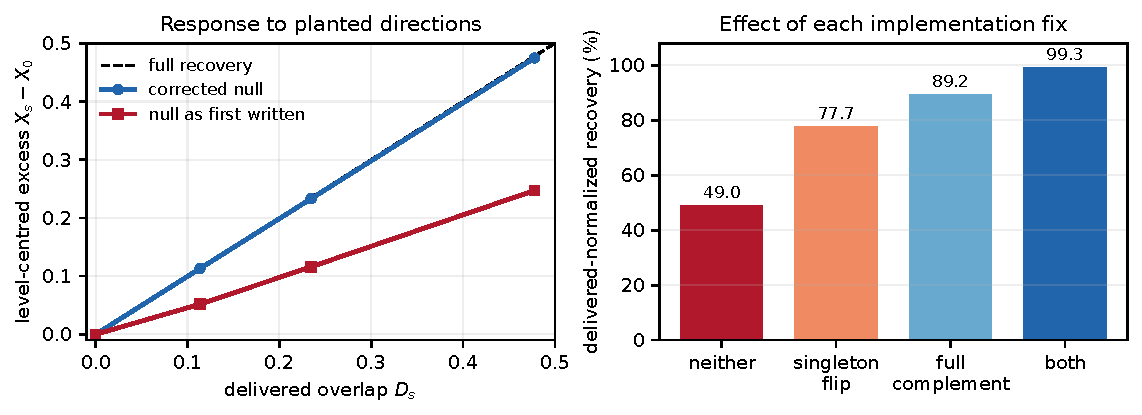
\includegraphics[width=\linewidth]{figures/fig_power.pdf}
\caption{Left: level-centred excess reported against overlap actually delivered by the positive
control. The diagonal is full recovery. Right: level-centred recovery at $s/k=1/4$ with each
activation-null correction enabled separately.}
\label{fig:power}
\end{figure}

\subsection{Power, measured by planting}
\label{sec:power}

The complement of the \texttt{H0} check is a positive control. Take a real task vector $A$ and a
partner $P_0$ drawn from the fitted null, then replace $s$ of the partner's top-$k$ read
directions with directions from $A$, projection/QR-complete the remaining directions, and retain
$P_0$'s singular values to obtain $P_s$ (exact operator in Appendix~\ref{app:power}). The
intervention introduces forced directional matches on top of the pair's pre-existing overlap;
finite-dimensional cross terms mean that it need not add exactly $s/k$.

We therefore normalise by what the intervention actually delivers. For candidate null
$\mathcal N$ define
\begin{align}
 D_s&=\mathbb E[\mathcal O(A,P_s)-\mathcal O(A,P_0)],\nonumber\\
 X_s^{\mathcal N}&=\mathbb E[\mathcal O(A,P_s)-
   \mathcal O(\mathcal N_1(A),\mathcal N_2(P_s))],\qquad
 R_s^{\mathcal N}=\frac{X_s^{\mathcal N}-X_0^{\mathcal N}}{D_s}.
 \label{eq:recovery}
\end{align}
Recovery is thus level-centred and uses delivered rather than nominal overlap. We run this
semi-synthetic stress test on real task vectors and the measured calibration covariance. The
plant preserves singular values but can change the block-occupancy profile on which the null
conditions, so $R_s$ measures sensitivity to this intervention after reconditioning; it is not
power against every possible cross-task dependence or evidence about how the conditioned
statistics arose.

Figure~\ref{fig:power} separates the two arms. The null as first written
recovers only $45.6$--$51.7\%$ of delivered overlap while returning $+0.00004$ at $s=0$, which
looks well behaved under the offset check; the corrected null recovers $99.3$--$99.6\%$ and has
$-0.000623$ at $s=0$. Both arms score the same planted pairs and differ only in the randomisation, which is the
combination we want: small reference offset and high response to the planted alternative. The
study covers four modules and one family of interventions, and planting can alter conditioned
occupancies, so we do not transfer the sub-percent deviation to the $72$-module observational
estimate.

\subsection{What the positive control found}
\label{sec:defects}

The diagnostic exposed two under-randomisation failures in the activation null: its fixed-rank
complement rotation reached only $4$--$18\%$ of that space, and it skipped singleton sign flips
although those directions carry $71\%$ of stored eigenvalue mass. The LoRA generator instead
matched only $\|B\|_F$, letting an uncontrolled factor spectrum set even the sign of its offset.
The zero-offset check missed the first two and had been declared rather than measured for the
third. Appendices~\ref{app:defects} and~\ref{app:ablation} give the fixes and ablation.

\subsection{A common-reference stress test for existing baselines}
\label{sec:baselines}

A reader's first instinct is to substitute some other transform for the isotropic comparator, so we
show how those transforms behave on pairs whose true overlap is zero by construction. We form
semi-synthetic pairs by independently applying our activation-conditioned generator to real
updates. None of the cited work proposes its transform as an evidential null; the rows are
candidate substitutions, not attributed claims. Residual orientation
coupling is absent by construction under this reference, while each endpoint retains its observed
spectrum and occupancy profile. Table~\ref{tab:baselines} reports each baseline's native excess;
these are diagnostics on a common input distribution, not one shared estimand, because whitening
changes the matrices being scored. Because our generator defines the reference, this experiment
neither independently validates our null nor establishes model-free false-positive rates.
\begin{table}[t]
\centering
\caption{Native excess on the same independent-orientation reference pairs, ViT-B/16, $k=8$,
eight fixed modules, and $20$ pairs per module ($160$ total; seed $0$). Exact orthogonality subtracts zero; isotropic subtracts $k/d$;
whitened rows use the participation-ratio floor or all $64$ stored directions before subtracting
$k/d$; the final three rows subtract their
own surrogate mean. Thus entries share overlap units but not an estimand.}
\label{tab:baselines}
\begin{tabular}{@{}lr@{}}
\toprule
baseline & reported excess \\
\midrule
exact orthogonality (no reference subtracted)        & $+0.0275$ \\
isotropic $k/d$                                     & $+0.0171$ \\
whitened at the participation ratio                 & $+0.0522$ \\
whitened, all stored directions                     & $+0.0554$ \\
generative activation model                         & $-0.8959$ \\
coordinate permutation (paired action)              & $-0.0000$ \\
\bottomrule
\end{tabular}
\end{table}

The untransformed reference pair's raw overlap is $0.0275$, or $2.6$ times isotropic chance;
subtracting the isotropic comparator reports $+0.0171$ excess. Whitening changes the scored
matrices and reports still larger native excesses
(Table~\ref{tab:baselines}). A transform introduced
to reduce interference inside a merge therefore need not be calibrated as an evidential baseline.

The mechanism is concentration, and it sharpens with the ridge. $C_H^{-1/2}$ amplifies small
eigendirections and drives both endpoints onto the same few of them: at a Tikhonov ridge of
$\lambda=10^{-4}\bar w$, $96.5\%$ of the whitened read mass lands on the twenty smallest stored
eigendirections, and a chance-overlap pair is reported at $0.7199$. RegMean's published
off-diagonal shrinkage $\alpha=0.9$ returns $0.0931$ on the same pair. Truncating the whitening at
the top $m_{\rm white}$ directions keeps the reference near chance ($0.0394$, $0.0405$, $0.0422$ at
$m_{\rm white}=8,32,64$), which is why we set $m_{\rm white}$ per module from its participation
ratio. The failure is therefore not whitening as such but whitening into directions the
calibration set does not determine.

The coordinate permutation is the useful counterexample. Here the same permutation is applied to
both endpoints, so overlap, and hence its offset, is exactly unchanged; this paired action is a
deliberate counterexample rather than the independent action in Eq.~\ref{eq:h0}. It nevertheless
destroys occupancy relative to fixed $C_H$, so \S\ref{sec:null} rejects it. Passing an offset check
is not sufficient, which is \S\ref{sec:level}'s lesson from the other side.

\subsection{The same test on the LoRA null}
\label{sec:lora-power}

For LoRA, we score only the attainable plant
$P_s^\star=P_sA^+A=(\alpha/r)B_sA$, with $B_s=(r/\alpha)P_sA^+$; both raw and null terms use
$P_s^\star$ (Appendix~\ref{app:lora-power}). It delivers $37.386\%$, $49.790\%$, and $57.043\%$ of the nominal affine increment
at $s=1,2,4$. Normalising the level-centred excess by those delivered increments gives
$101.117\%$, $101.078\%$, and $100.701\%$ recovery. The initial norm-matched generator also has
near-$100\%$ level-centred response, but its unplanted level is $-0.1485$, versus $-0.0073$ after
factor-spectrum matching. The correction therefore calibrates level rather than rescuing low
power or an upward bias. This remains one intervention over four modules and six tasks.


\section{Experiments}
\label{sec:exp}

\paragraph{Setup.}
We evaluate CLIP vision encoders fine-tuned on the task-arithmetic benchmark of
\citet{ilharco2023editing} as extended to twenty tasks by \citet{wang2024localizing}: all $190$
pairs over all $72$ linear modules for each ViT-B encoder, and $48$ \texttt{q}/\texttt{v} modules
for ViT-L/14.
$C_H$ comes from $1001$ images drawn round-robin across seven of the benchmark's own datasets on
the frozen base; a separate rebuilding record stores source counts, fold membership, and hashes.
All substantive overlap results use $k=8$. For whitening comparisons we truncate at the module's
participation ratio $m_{\rm white}$; the activation null retains $m_C=64$ eigendirections and
reads its rotation blocks from the eigenvalue standard errors as in \S\ref{sec:method}.
The calibration composition, not the calibration draw, is what moves the answer: a deliberately
different balanced MNIST/Cars/SVHN mixture gives $21.482\%$ ($-3.863$ points) while two
source-stratified refits at fixed source counts shift it by at most $0.243$ points
(Appendix~\ref{app:calibration}). The residual stays positive in both controls.
Brackets are finite-pool stability intervals, the $2.5$th and $97.5$th percentiles of $50{,}000$
crossed task--layer resampling replicates (seed $20260915$). They describe sensitivity to
reweighting the observed tasks and layers, not superpopulation coverage, and condition on one
checkpoint per task, fixed calibration and blocking, and the exact scalar null (or the pooled
$64$-draw Monte Carlo null for adapter arms). The external-reference \texttt{H0} is a separate
stress diagnostic and is never added to an estimate.

\begin{figure}[t]
\centering
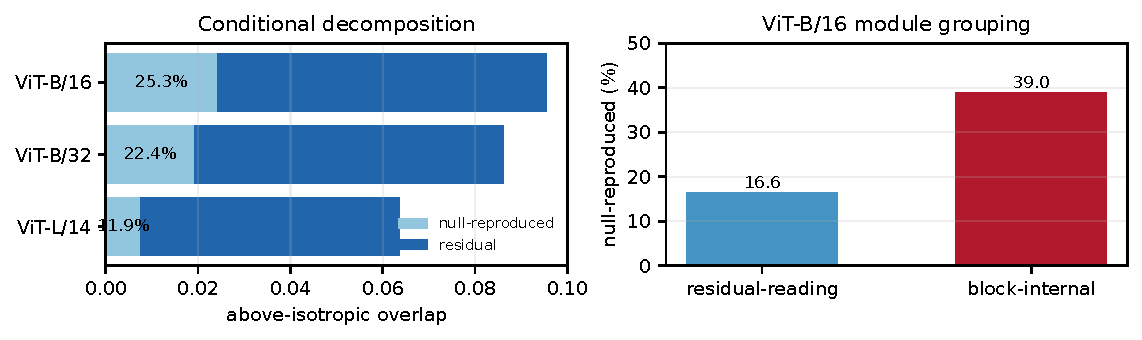
\includegraphics[width=\linewidth]{figures/fig_main.pdf}
\caption{Left: above-chance overlap split into the part the activation null reproduces and the
residual for each encoder. Right: an exploratory ViT-B/16 split by whether a module reads the
residual stream or a representation built within its block. All fractions use the null expectation
without adding the realised \texttt{H0} diagnostic.}
\label{fig:main}
\end{figure}

\subsection{Full fine-tuning: the conditional null reproduces about a quarter}
\label{sec:fullft}

In the two complete ViT-B measurements, the activation-conditioned null reproduces
$25.3451\%$ ($[19.3033,31.8010]$) and $22.3961\%$ ($[15.5516,29.8850]$) of above-isotropic
top-$8$ overlap. The partial ViT-L/14 \texttt{q}/\texttt{v} measurement gives $11.8961\%$
($[8.1064,16.4895]$).
Conditional on the fixed
null specification, the residual is positive under crossed task--layer resampling, but
should not automatically be identified with
task-derived sharing: it is directional agreement not accounted for by the conditioned
statistics. An earlier implementation put its headline reproduced fraction near $67\%$; the positive
control in \S\ref{sec:validate} shows why we reject it, with delivered-signal recovery of only
$45.6$--$51.7\%$ instead of the corrected null's $99.3$--$99.6\%$.

Module role, not architecture, is where the fraction actually moves, and the pooled headline hides
it. Figure~\ref{fig:main} shows the grouping: the exact null reproduces $16.6\%$ for ViT-B/16
modules reading the residual stream and $39.0\%$ for modules reading a representation built within
the block. Width carries part of that gap, since \texttt{fc2} has four times the input width and
supplies $81.9\%$ of the block-internal group's numerator. Holding width fixed leaves
\texttt{out\_proj} at $26.2\%$ against $16.1\%$ for attention \texttt{q}/\texttt{k}/\texttt{v}, so
roughly $10$ of the $22$ points survive as a role effect. One possible explanation is that
task-specific structure accumulates in the residual stream, whereas \texttt{out\_proj} and
\texttt{fc2} read representations more tightly constrained by the block.

The pooled ratio is a design-weighted blend, and its spread matters for how the headline is read.
Across the $72$ ViT-B/16 modules the reproduced fraction runs from $0.4\%$ to $65.1\%$ with median
$19.1\%$, and $394$ of $13{,}680$ cells have a negative residual. So $25.3\%$ is a property of this
module inventory, not of a typical module, and a different inventory would move it.

\begin{table}[h]
\centering
\caption{Cross-task read-subspace overlap and its scalar decomposition. Complete encoder pools use
all $190$ task pairs; the matched eight-task row uses all $28$. \texttt{raw} is
Eq.~\ref{eq:overlap}, \texttt{iso} is $k/d$, and \texttt{null} is the exact expectation in
Eq.~\ref{eq:null-expectation}. Terms are averaged before the ratio, and no Monte Carlo draw enters
these scalar results. The last column restricts every pool to \texttt{q} and \texttt{v}, the only
module set all three encoders share.}
\label{tab:main}
\small
\setlength{\tabcolsep}{4pt}
\begin{tabular}{@{}lrrrrrrr@{}}
\toprule
& modules & \texttt{raw} & \texttt{iso} & \texttt{null} & residual & reproduced & $q/v$ only \\
\midrule
ViT-B/16 & $72$ & $0.104574$ & $0.009115$ & $0.033309$ & $0.071265$ & $25.3\%$ & $14.7\%$ \\
ViT-B/32 & $72$ & $0.095313$ & $0.009115$ & $0.028420$ & $0.066893$ & $22.4\%$ & $13.5\%$ \\
ViT-L/14 $q/v$ & $48$ & $0.071402$ & $0.007813$ & $0.015377$ & $0.056024$ & $11.9\%$ & $11.9\%$ \\
matched FT8 $q/v$ & $24$ & $0.089930$ & $0.010417$ & $0.023333$ & $0.066597$ & $16.2\%$ & $16.2\%$ \\
\bottomrule
\end{tabular}
\end{table}

Table~\ref{tab:main} gives the terms behind these fractions, and its last column shows that most
of the apparent spread across encoders is module selection. ViT-L/14 is instrumented on \texttt{q}
and \texttt{v} only; restricting the two ViT-B pools to the same two module types moves them to
$14.7\%$ and $13.5\%$, so a $13.5$-point gradient becomes a $2.8$-point one. We therefore do not
read Table~\ref{tab:main} as an architecture trend. The fraction is also specification-dependent:
across $m_C\in\{16,32,64\}$ and $z\in\{1,2,3\}$ at $k=8$ it spans $20.22$--$25.61\%$ for ViT-B/16,
and $13.28$--$30.37\%$ once $k$ is swept as well, which changes the statistic rather than its
estimate (Appendix~\ref{app:calibration}).

The residual's sign is not in question and the resampling does not test it: every one of the $12$
layer margins ($\ge 0.0334$) and all $20$ task margins ($\ge 0.0282$) are strictly positive, so a
nonnegative reweighting cannot produce a negative replicate. What the intervals describe is width.
For ViT-B/16, ViT-B/32, and ViT-L/14 the crossed-resampling residual intervals are
$[+0.04540,+0.10568]$, $[+0.04224,+0.10085]$, and $[+0.03476,+0.08252]$. Within each replicate,
independent multinomial endpoint counts $C_t$ and layer counts $L_\ell$ give row weight
$C_aC_bL_\ell$; all module types in a layer stay together, weighted means precede the ratio, and
external \texttt{H0} diagnostics remain separate.

No single task or layer carries the result. Dropping one task at a time moves the reproduced
fraction within $24.685$--$25.896\%$, $21.856$--$22.939\%$, and $11.310$--$12.165\%$ for the three
encoders; dropping one layer at a time gives $24.359$--$28.411\%$, $21.272$--$26.392\%$, and
$10.955$--$13.587\%$. Every residual stays positive in every leave-one-out cell. The layer ranges
are the wider of the two, which is what the module-role split above predicts: layers differ in how
much of their width reads the residual stream.

\subsection{Low-rank adapters: a shared-start-compatible signature}
\label{sec:lora}

Low-rank adapters make the regime-specific conditioned object explicit. Since
$\mathrm{row}(BA)\subseteq\mathrm{row}(A)$, shared $A_0$ imposes a common admissible row space;
this remains exact when $A$ is frozen, while for trained $A$ we measure rather than assume it.
Across all $24$ targeted modules in the factor audit (Appendix~\ref{app:lora-factors}),
learned-from-zero $B$ overlaps at $0.0540$--$0.0570$, well below $A$'s
$0.8759$--$1.0000$ but still about five times chance. The
linearized pool, with bit-identical frozen $A$, has the highest $A$ and product overlap.
Almost all of that overlap is the rank constraint, and the null adds little to saying so. The
following pool-level estimates use all $24$ targeted modules and eight tasks. For LoRA-16 the
$A$-conditioned factor null reproduces $80.3\%$ ($[75.7,85.1]$) of above-isotropic overlap, and the
linearized pool $76.1\%$ ($[72.2,80.2]$). But a shared $A$ confines both updates to one
$r$-dimensional row space, where two independent top-$k$ subspaces already agree at $k/r$, and the
one-line comparator $(k/r-k/d)/(\overline{\texttt{raw}}-k/d)$ gives $82.0\%$ and $74.8\%$ on the same
pools. Conditioning on observed $A$ and on $B$'s spectrum therefore moves the answer by $1.7$ and
$1.3$ points. Under a shared start the admissible row space accounts for nearly all observed
product-subspace overlap, and the factor null confirms that rather than discovering it. Its
attainable plant delivers $37.4/49.8/57.0\%$ of the nominal increment with level-centred recovery
$101.1/101.1/100.7\%$ at $s=1/2/4$, so the construction is calibrated.

Full fine-tuning over the same $24$ modules gives $16.2\%$ ($[9.2,27.5]$). We do not read the gap
against $80.3\%$ as one contrast: they are ratios with different denominators, computed under nulls
that condition on different objects.

\paragraph{A regime-mismatched null changes the attribution.}
The activation null instead leaves $99.9\%$ of the same LoRA pool's above-chance overlap as
residual, versus $19.7\%$ under the observed-$A$-preserving factor null ($+0.5966$ versus
$+0.1176$). It answers a different question because it does not hold observed $A$ fixed;
transferring a null across regimes therefore changes the inferred effect size substantially.

\subsection{Consequences: attribution rather than a new merge}
\label{sec:projector}
\label{sec:merge}
\label{sec:ranking}
We rebuild the null-space projector of \citet{qiu2026nufilt} from real and independently
randomised task vectors (Appendix~\ref{app:projector}). Observed--null basis overlap is $0.8750$
versus $0.0208$ chance for LoRA and $0.2594$ versus $0.1667$ for full fine-tuning. The corresponding
basis mass in the top activation subspace is $0.1356$ and $0.2612$ (chance $0.0833$); none of
these projector statistics has a dedicated positive control. This does not test projector utility.
A separate cross-term-only compression heuristic does not beat the cumulative-update basis at any
rank budget, losing on $6$ to $8$ of the eight tasks from $r=32$ upward and tying within noise at
$r=8$ (Appendix~\ref{app:merge}). Calibration is also nearly rank-preserving over task pairs
(Spearman $0.994$--$0.995$); we do not test a retrained mergeability predictor. The contribution
is therefore inferential: a large effect or useful basis does not by itself establish the
mechanism invoked to explain it.

\section{Discussion}

Cross-task top-$8$ sharing remains positive after conditioning in every fully fine-tuned CLIP pool,
but its attribution changes. The null reproduces $25.3\%$ and $22.4\%$ in the complete ViT-B runs;
the factor-conditioned LoRA value is $80.3\%$, with near-full recovery of delivered signal in its
narrow positive control. These quantities split agreement under stated conditions; they do not
locate its origin in the base or the shared start.

A reader should report a null's invariants, training regime, reference offset, and positive-control
response. Here conditioning changes effect size while pair rankings barely move, and a separate
coupling-only basis does not improve merge accuracy. A structural claim is only as specific as the
null it survives and only as credible as that null's measured response.

\section*{Reproducibility Statement}
Appendix~\ref{app:repro} records task pools, calibration data, numerical settings, and checks;
the supplementary artifact provides row-level results, executable analysis, and manifests.
\section*{Use of Large Language Models}
Large language models were used for methodology and experiment feedback, code implementation,
mathematical and numerical checking, result interpretation, figure and artifact preparation, and
drafting and editing. The authors reviewed and tested the resulting work and take full
responsibility for the paper's content.

\bibliography{iclr2027_conference}
\bibliographystyle{iclr2027_conference}
\appendix
\section{Limitations and future work}
\label{app:limits}

All quantitative conclusions concern CLIP vision encoders. The headline uses $k=8$, $m_C=64$,
and the $2\sigma$ resolution convention; we sweep $k$, $m_C$, and the resolution multiplier below.
ViT-L/14 covers only \texttt{q} and \texttt{v}, and $C_H$ is estimated from seven of the twenty
benchmark datasets under one recorded mixture. One deliberately different composition is tested
below; broader calibration compositions and language models remain open.
The reported finite-pool stability intervals hold the calibration draw, fold partition, block
rule, and $m_C$ fixed; they do not incorporate uncertainty from estimating or selecting the null.
They are not superpopulation coverage statements: each task contributes one checkpoint/training
realisation, so training-run and checkpoint variation are unmeasured.
Scalar activation-null values use Eq.~\ref{eq:null-expectation} exactly; adapter intervals hold
their pooled $64$-draw realised Monte Carlo null values fixed. We draw $50{,}000$ crossed
task--layer resampling replicates. Independent multinomial endpoint counts $C_t$ and layer counts $L_\ell$
give each row weight $C_aC_bL_\ell$; all module types within a selected layer remain grouped.
Each replicate takes the ratio after weighted averaging. The pseudorandom seed is $20260915$.
As a finite-pool influence check for the exact activation arms, leave-one-task-out reproduced
fractions range $24.685$--$25.896\%$, $21.856$--$22.939\%$, and $11.310$--$12.165\%$ for
ViT-B/16, ViT-B/32, and ViT-L/14; the corresponding leave-one-layer-out ranges are
$24.359$--$28.411\%$, $21.272$--$26.392\%$, and $10.955$--$13.587\%$. Every residual remains positive.

The raw outer-product gradient identity involves activations along each fine-tuning trajectory
and, under scalar-step gradient descent, constrains the update to their span. Our null instead
conditions on the frozen base's second moment. Feature drift, adaptive coordinatewise
preconditioning, and weight decay break an exact passage between those statements. Consequently,
the activation-conditioned decomposition is descriptive: its post-fine-tuning occupancy profile
can include learned structure, and identifying its origin would require an intervention or an
additional stability assumption that we do not test.

The LoRA result is limited to rank $16$, one shared-start protocol, eight tasks, and the reported
attention modules. Its factor null preserves $A$ and the singular spectrum of $B$, not the
product spectrum of $BA$. In a four-module, six-task stress test the attainable plant delivers
$37.4$--$57.0\%$ of its nominal increment, and the null recovers $100.7$--$101.1\%$ of that
delivered signal. This establishes level and response only for that planting operator; the
$87.5\%$ projector-basis fraction has no dedicated positive control. A controlled
shared-versus-independent-$A_0$ experiment is absent, and $B$ remains about five times above
isotropic chance. Finally, calibration is nearly rank-preserving and the cross-term basis does
not improve compressed-merge accuracy; the evidence supports measurement and attribution claims,
not a better merging algorithm.

\section{Invariants of the overlap statistic}
\label{app:invariants}

Every numerical property below is checked directly in the analysis; these checks should accompany
the released measurement code rather than be inferred from library defaults.

Beyond the scalar occupancies and energies in \S\ref{sec:null}, the group action fixes
$\Delta W_iP_b\Delta W_i^\top$ and the eigenvalues of
$V_i^{(k)\top}P_bV_i^{(k)}$ for every block. The former contains output-side block Gram geometry
and the latter its principal-angle spectrum. A looser null conditioning only on $t_{ib}$ could
therefore give a different attribution.

\paragraph{Why Eq.~\ref{eq:null-expectation} is exact.}
Haar averaging within block $b$ gives
$\mathbb E[Q_i^\top\Pi_iQ_i]=\sum_b(t_{ib}/d_b)P_b$, where
$d_b=\operatorname{rank}(P_b)$. For independent task-wise draws, linearity and
$P_bP_c=\mathbf 1\{b=c\}P_b$ give
$\mathbb E\operatorname{tr}(Q_i^\top\Pi_iQ_iQ_j^\top\Pi_jQ_j)
=\sum_b t_{ib}t_{jb}/d_b$; division by $k$ yields Eq.~\ref{eq:null-expectation}.

\begin{itemize}
\item \textbf{Orientation.} \texttt{top\_right} returns the right singular vectors, of shape
$(d_{\mathrm{in}}, k)$, matching an explicit SVD on a rectangular matrix where a transpose would
be silent. The convention $\Delta W = U S V^\top$ puts $V$ on the input side; swapping it
reverses every conclusion in this paper.
\item \textbf{Normalisation.} $\mathcal{O}(A,A)=1$ to $10^{-6}$, and two independent uniformly
random $k$-subspaces average $0.03995$ against $k/d = 0.04000$ over $300$ draws. We confirm the
same identity at $(d,k) \in \{(200,8),(200,32),(400,8),(3584,8),(100,10)\}$.
\item \textbf{Degenerate inputs are refused.} The SVD of a zero matrix returns an arbitrary
orthonormal basis, and returns the \emph{same} one each time, so two zero task vectors score
$\mathcal{O}=1.0000$. In a LoRA checkpoint every module the adapter does not target is exactly
zero, so an unguarded run over an adapter pool fills its averages with the maximum possible
value taken from modules that did not change. \texttt{top\_right} raises on such an input and
the caller drops and counts those cells.
\item \textbf{Checkpoint reads.} Weights are read by matching module paths to checkpoint keys by
suffix, since \texttt{CLIPVisionModel.named\_modules()} yields \texttt{encoder.layers.0...}\ while
the checkpoint stores \texttt{vision\_model.encoder.layers.0...}. A suffix matching more than one key is refused: the full CLIP checkpoint holds both
\texttt{text\_model.*} and \texttt{vision\_model.*} under identical suffixes, and picking either
silently would build task vectors from the text tower and compare them against a vision
covariance. Tensors returned this way are bit-identical to a \texttt{state\_dict} load.
\end{itemize}

\section{Calibration choices for whitening and activation blocks}
\label{app:calibration}

\paragraph{Block-error rule.}
Partition the calibration set into eight disjoint folds and compute the ordered covariance
eigenvalues $\lambda_j^{(f)}$ independently on each fold. With their mean $\bar\lambda_j^{F}$,
the implementation uses the split-sample standard error
$\sigma_j=[\sum_{f=1}^{8}(\lambda_j^{(f)}-\bar\lambda_j^{F})^2/(8\cdot7)]^{1/2}$.
The blocks are the transitive consecutive components induced by overlap of adjacent
$\widehat\lambda_j\mathbin{\pm}2\sigma_j$ intervals, where $\widehat\lambda_j$ is the eigenvalue
from the full calibration pool. This is an operational coarsening, not a confidence interval for
eigenspace identifiability.

\paragraph{Finite calibration refits.}
Holding the seven source counts and extraction procedure fixed, two source-stratified bootstrap
refits (seeds $20260916$ and $20260917$) give full ViT-B/16 exact reproduced fractions
$25.102\%$ and $25.302\%$, versus the $25.345\%$ headline, for a maximum $0.243$-percentage-point
shift. This is the observed range of two refits, not a calibration confidence interval, and does
not test a different source composition.

\paragraph{Composition stress control.}
Separately, we sample without replacement from deterministic test splits to balance $334$ MNIST,
$334$ Stanford Cars, and $333$ SVHN images (seed $20260919$). This deliberately different
calibration gives exact ViT-B/16 null $0.029621$, residual $0.074953$, and reproduced fraction
$21.482\%$, or $3.863$ percentage points below the seven-source headline. Holding this covariance
fixed, the crossed finite-pool stability intervals are $[16.8975,26.2690]\%$ for the fraction and
$[+0.048606,+0.109015]$ for the residual. The median participation ratio is $12.691$, with
$71/72$ modules below $64$, so both composition and spectral effective rank have changed. This is
a stress control, not an estimate of calibration uncertainty or an interval over possible compositions.

A complementary post-hoc stratification asks whether zero, one, or both endpoints of a task pair
belong to the seven calibration sources ($78/91/21$ pairs). The reproduced fractions rise from
$23.06/26.56/28.33\%$ for ViT-B/16, $20.38/23.45/24.55\%$ for ViT-B/32, and
$10.20/12.64/14.47\%$ for ViT-L/14; the residual remains positive in every cell. This gradient is
consistent with composition sensitivity, but it does not isolate calibration membership from task
identity and is not used for inference.

\paragraph{Truncation.} Whitening two task vectors by a shared $C_H$ manufactures overlap when
it is aggressive. On independent task vectors whose true overlap is chance ($0.0400$), a
Tikhonov ridge at $\lambda = 10^{-4}\bar{w}$ returns $0.7199$ and RegMean's published
off-diagonal shrinkage $\alpha = 0.9$ returns $0.0931$. The mechanism is that $C_H^{-1/2}$
amplifies small eigendirections and drives both task vectors onto the same few of them: at
$\lambda = 10^{-4}\bar{w}$, $96.5\%$ of the whitened read mass lands on the twenty smallest
stored eigendirections. Whitening only the top $m_{\rm white}$ directions keeps reference overlap
near chance ($0.0394$, $0.0405$, $0.0422$ at $m_{\rm white}=8,32,64$).

We set $m_{\rm white}$ per module from that module's participation ratio
$(\sum_i w_i)^2 / \sum_i w_i^2$, used here as an operational effective-rank truncation. In our
calibration refits, directions beyond this cutoff were unstable; the participation ratio is not
an identifiability threshold. The ratio must be computed from the full spectrum:
taken over only the $m_C$ retained eigenvalues it is bounded above by
$m_C$ by Cauchy--Schwarz, which understates it and makes any gate comparing
the two a tautology.

\paragraph{Why a block count was rejected.} \S\ref{sec:method} sets the rotation blocks from
what the calibration data can resolve. We record here what the alternative looked like, because
the alternative is what a reader would reach for first.

Fixing a block count and complement rotation rank leaves two choices that no invariant selects,
and the answer moves with them: sweeping the rotation rank of the complement from $32$
to $512$ moved the reproduced fraction from $48\%$ to $23\%$ under the null as it then stood.
Subtracting that null's offset on a constructed reference did not stabilise it. The
resolution-based construction eliminates those two outcome-sensitive choices, since the
complement is a single unresolved block and is rotated in full. It does not eliminate design
choices: the uncertainty multiplier, fold-SE scheme, calibration sample, and stored dimension
remain part of the null specification.

The sweep is also where the defect of \S\ref{sec:defects} hid in plain sight. A rotation rank
that changes the answer by a factor of two is a rotation rank that is destroying different
amounts of structure, and the endpoint the construction actually calls for, rotating the whole
complement, lies outside the range that was swept.

\paragraph{Block structure is a function of the calibration budget.}
Blocks are the groups of eigendirections that our operational interval rule treats as unresolved.
They tend to sharpen as the calibration set grows: estimated eigenvalue errors contract, so fewer
adjacent intervals overlap and blocks split. This behavior does not make interval overlap a
confidence theorem for eigenspace identifiability.
The first three columns below are measured on nested subsets of one image pool. At each budget we
partition images into eight disjoint folds and compute the eight foldwise eigenvalue replicates
used by the split-sample rule in \S\ref{sec:method}. The remainder scales the measured standard errors,
the pool having stopped at $1001$.

\begin{table}[h]
\centering
\begin{tabular}{@{}lrrrcrrr@{}}
\toprule
& \multicolumn{3}{c}{measured} & & \multicolumn{3}{c}{extrapolated} \\
\cmidrule(r){2-4}\cmidrule(l){6-8}
calibration images & $224$ & $500$ & $1001$ & & $2000$ & $5000$ & $\infty$ \\
\midrule
ViT-B/16 & $16$ & $25$ & $37$ & & $46$ & $55$ & $64$ \\
ViT-B/32 & $15$ & $21$ & $37$ & & $44$ & $55$ & $64$ \\
\bottomrule
\end{tabular}
\end{table}

This is a resource-resolution trade-off that the method makes visible. Too few images and the blocks are coarse, the
null rotates across gaps that are in fact resolved, and its constructed-reference offset grows.
As the budget grows, the rule tends to split blocks. Under a simple population spectrum and fixed
$m_C=64$, its retained-region limit is $\{\pm1\}^{64}$ while the unresolved complement remains
$O(d_{\rm in}-64)$. Thus the limit is not the identity: signs randomise off-diagonal terms within
the retained region, and the complement is fully rotated. It has no power against agreement
expressed only as shared retained-axis occupancy, while retaining power against sign-sensitive or
complement orientation alignment. The $\infty$ column extrapolates the retained block count only;
it is not a measured power result.

The budget matters for a reason that is visible in the block counts themselves. A run at $224$
images drawn independently of the pool above resolved $13$ and $11$ blocks where the nested $224$
subset resolves $16$ and $15$, so at that budget the block structure is not stable across draws
of the calibration set, let alone across architectures. At $1001$ the two architectures happen
to agree at a median of $37$ blocks and the same median largest block. This is a useful
cross-architecture check, not proof of sampling stability. The calibration budget is part of the
measurement specification and must be fixed and reported.

The reproduced fraction is not reported against the budget, since the two budgets were measured
under nulls that differ by more than the budget: the $224$-image run predates the corrections
of \S\ref{sec:defects}, so comparing them would charge the calibration set for a change that
belongs to the null.

\paragraph{Where the blocked region ends.}
The activation-null stored dimension $m_C$ divides the space the null treats two ways: inside
$\mathrm{span}(V)$ it rotates within resolvable blocks, outside it rotates in full. We sweep
$k\in\{4,8,16,32\}$, $m_C\in\{16,32,64\}$, and uncertainty multiplier
$z\in\{1,2,3\}$ on each reported pool:

\begin{table}[h]
\centering
\begin{tabular}{@{}lrr@{}}
\toprule
pool & $k=8$, all $(m_C,z)$ & full $(k,m_C,z)$ grid \\
\midrule
ViT-B/16 & $20.22$--$25.61\%$ & $13.28$--$30.37\%$ \\
ViT-B/32 & $17.94$--$22.55\%$ & $13.31$--$28.51\%$ \\
ViT-L/14 $q/v$ & $5.84$--$12.00\%$ & $5.36$--$19.01\%$ \\
\bottomrule
\end{tabular}
\end{table}

At fixed $(k,m_C)$, the largest observed change from varying $z$ is $0.754$ percentage points; most of
the fixed-$k$ range comes from $m_C$. This is variation in the conditional estimand---storing more
directions changes what the null holds fixed---rather than numerical instability of its exact
estimator. We pre-specify the headline at $m_C=64,z=2$; $m_C$ remains distinct from the per-module
whitening truncation $m_{\rm white}$ above.

\paragraph{The calibration must use the observed spectrum.} The reference offset is not a property
of the null alone; it depends strongly on the spectrum of the task vectors the null is
calibrated against. Substituting a synthetic exponential spectrum for the observed one raises
the realised reference offset at eight blocks from $+0.0041$ to $+0.0254$, a factor of six.
This sensitivity is another reason not to transfer that diagnostic into the estimand.
The reason is that real task
vectors have rapidly decaying spectra, which makes the top-$k$ subspace well determined and the
block rotation effective, whereas a flat spectrum leaves that subspace ill-determined and the
block structure dominates. A null calibrated against a spectrum the data does not have
calibrates the wrong quantity.

\section{LoRA factor audit}
\label{app:lora-factors}

\begin{table}[h]
\centering
\caption{ViT-B/16, eight tasks, $28$ pairs, all $24$ targeted attention modules; all entries use top-$8$ singular
subspaces. $B$ is initialised at zero and is therefore entirely learned; $A$ is not.
\texttt{lin-LoRA} is the partial linearization of \citet{tang2024linearization}, which leaves
$A$ bit-identical across tasks.}
\begin{tabular}{@{}lrrr@{}}
\toprule
& $A$ right & $B$ left & $\Delta W$ right \\
\midrule
LoRA-16   & $0.8759$ & $0.0540$ & $0.6075$ \\
lin-LoRA  & $1.0000$ & $0.0570$ & $0.6649$ \\
isotropic & $0.0104$ & $0.0104$ & $0.0104$ \\
\bottomrule
\end{tabular}
\end{table}

At the $k=8$ boundary, the relative singular gap
$(s_8-s_9)/s_8$ is above $10^{-3}$ for every observed $A$ and $BA$ cell in both
eight-task, $24$-module adapter pools.  Across $24{,}576$ factor-null $BA$ redraws, only four
fall below $10^{-3}$ and none below $10^{-4}$; the median gap is about $0.099$ in each arm.
Thus exact or numerical cutoff ties do not drive the aggregate factor-null result, although the
finite-$k$ choice remains part of the estimand.

\section{Power of the LoRA null}
\label{app:lora-power}

\begin{table}[h]
\centering
\caption{A rank-$16$ LoRA stress test, ViT-B/16, four attention modules, six tasks. The fitted
factor null has pre-planting overlap $\mathcal O_0=0.4825$. From an unconstrained plant $P_s$ we
form the attainable $P_s^\star=P_sA^+A=(\alpha/r)B_sA$, where
$B_s=(r/\alpha)P_sA^+$. Both raw and null terms score $P_s^\star$. Delivery divides
$\Delta\mathrm{raw}$ by $(s/k)(1-\mathcal O_0)$; recovery is level-centred as in
Eq.~\ref{eq:recovery}.}
\label{tab:lora-power}
\begin{tabular}{@{}lrrrrr@{}}
\toprule
planted & raw & delivery & initial $X_s$ & corrected $X_s$ & recovery \\
\midrule
$0/8$ & $0.4825$ & ---        & $-0.1485$ & $-0.0073$ & --- \\
$1/8$ & $0.5067$ & $37.386\%$ & $-0.1243$ & $+0.0172$ & $101.117\%$ \\
$2/8$ & $0.5469$ & $49.790\%$ & $-0.0840$ & $+0.0579$ & $101.078\%$ \\
$4/8$ & $0.6301$ & $57.043\%$ & $-0.0009$ & $+0.1414$ & $100.701\%$ \\
\bottomrule
\end{tabular}
\end{table}

The initial norm-matched generator also has approximately $100\%$ level-centred response, but a
large $s=0$ error. Spectrum matching changes that level from $-0.1485$ to $-0.0073$ while
retaining near-full response. The correction therefore fixes level; it is not evidence that the
initial null had low power or upward bias. Values just above $100\%$ reflect finite draws.

\section{Merged accuracy by rank budget}
\label{app:merge}

\begin{table}[h]
\centering
\caption{Merged accuracy averaged over the eight tasks, ViT-B/32, $500$ test images per task,
update compressed to rank $r$. Zero-shot is $38.9\%$ and uncompressed task arithmetic is
$59.5\%$.}
\label{tab:merge}
\begin{tabular}{@{}lrrrrrr@{}}
\toprule
rank $r$ & $8$ & $16$ & $32$ & $64$ & $128$ & $256$ \\
\midrule
$\tau$ basis        & $45.9$ & $49.9$ & $52.8$ & $55.7$ & $57.6$ & $59.0$ \\
cross-term basis    & $45.3$ & $48.8$ & $51.4$ & $53.5$ & $54.8$ & $55.7$ \\
\bottomrule
\end{tabular}
\end{table}

The separate cross-term-only heuristic uses
$\sum_{t\ne s}\Delta W_t^\top\Delta W_s=\tau^\top\tau-
\sum_t\Delta W_t^\top\Delta W_t$. This does not improve compressed-merge accuracy: the
$\tau$ basis wins at every tested budget, the gap widens with
$r$, and at $r=256$ it wins on all eight tasks separately. Concentrating empirical cross-task
coupling is therefore insufficient for better compressed-merge accuracy in this experiment.

Calibration is close to rank-preserving. Across the $190$ ViT-B/32 pairs, raw and calibrated
overlap have Spearman $0.995$ and share $17$ of the top $20$ pairs; ViT-B/16 gives $0.994$ and
shares $19$ of the top $20$. Thus an ordering-only consumer receives nearly the same ordering on these pools,
although we do not retrain the mergeability predictor of \citet{demystify2026}.

\section{Estimating $C_H$}
\label{app:cov}

$C_H$ is $d_{\mathrm{in}} \times d_{\mathrm{in}}$, which is $1.4$ GB per module at
$d_{\mathrm{in}} = 18944$ and infeasible to store across a network.
For the vision encoders studied here the exact matrix is affordable ($594$ MB across all $72$
modules of ViT-B/32) and we use it.
For larger models we provide a two-pass estimator: a Frequent Directions sketch locates the
subspace, and a second pass accumulates the exact $m_C \times m_C$ second moment inside it.
The second pass is necessary. Frequent Directions biases eigenvalues
downward by construction, and whitening applies $C_H^{-1/2}$, so an understated eigenvalue is an
over-amplified direction; on synthetic data at sketch size $128$ the eigenvalue error falls from
$0.49$ to $0.0016$ between the two passes while the top-$8$ subspace agreement is $0.998$
either way.

\paragraph{The calibration set is part of the measurement.}
$C_H$ is an expectation over some input distribution, and the answer depends on which.
We draw it from a mixture across several of the benchmark's own datasets, since a single one
would make $C_H$ the base geometry \emph{on that task's inputs} and
reintroduce the conditioning the test exists to remove.
A separate rebuilding record lists all image identifiers, per-source counts, hashes, and fold
memberships, while each covariance manifest records its item count and a basename--byte-size
hash. We verified that the two records enumerate the same $1001$ basenames; the release links
them explicitly rather than implying that source labels are embedded in each flattened
covariance manifest. The covariances themselves come to $26$ GB and need not be distributed; a
reproducibility artifact must include this rebuilding record and the extraction commands.

\section{Reproducibility record}
\label{app:repro}

\paragraph{Checkpoints and task pools.}
The frozen bases are \texttt{openai/clip-vit-base-patch16},
\texttt{openai/clip-vit-base-patch32}, and \texttt{openai/clip-vit-large-patch14}. Full-fine-tuned
specialists follow \texttt{tanganke/<architecture>\_<task>}. The $20$ task labels are
\texttt{cifar10}, \texttt{cifar100}, \texttt{dtd}, \texttt{emnist\_letters}, \texttt{eurosat},
\texttt{fashion\_mnist}, \texttt{fer2013}, \texttt{food101}, \texttt{gtsrb}, \texttt{kmnist},
\texttt{mnist}, \texttt{oxford-iiit-pet}, \texttt{oxford\_flowers102}, \texttt{pcam},
\texttt{rendered-sst2}, \texttt{resisc45}, \texttt{stanford-cars}, \texttt{stl10},
\texttt{sun397}, and \texttt{svhn}. The matched eight-task comparison uses \texttt{dtd},
\texttt{eurosat}, \texttt{gtsrb}, \texttt{mnist}, \texttt{resisc45}, \texttt{stanford-cars},
\texttt{sun397}, and \texttt{svhn}; its adapter repositories append \texttt{\_lora-16} or
\texttt{\_l-lora-16}. Rank and scale are read from each \texttt{adapter\_config.json}, and
untargeted modules are dropped rather than treated as zero subspaces.

\paragraph{Calibration and numerical settings.}
The rebuilding record contains $143$ images from each of \texttt{cifar10}, \texttt{dtd},
\texttt{eurosat}, \texttt{gtsrb}, \texttt{resisc45}, \texttt{stl10}, and \texttt{sun397}; fold
sizes are $126,125,125,125,125,125,125,125$. Images are the first valid examples encountered in
the streaming training split of each \texttt{tanganke/<source>} dataset, converted to RGB.
Extraction uses each model's \texttt{CLIPImageProcessor}, all sequence tokens (class and patch), exact uncentred
$\sum h h^\top/n$ accumulation in float32, $m_C=64$, and CPU execution. The extractor-input
basename/size hash common to the three covariance manifests has prefix \texttt{8f88002f7557}; the separate logical image/fold
record has identifier-list-hash prefix \texttt{73797f525986}. Full digests are in the artifact.

\paragraph{Randomisation and verification.}
The activation-null scalar results are the exact expectation in Eq.~\ref{eq:null-expectation};
they use no random draws. On the matched full-fine-tuning pool, a sampled check gives null
$0.02330$ versus exact $0.02333$. External-reference diagnostics use finite draws, the two
factor-null adapter arms use four independent $16$-draw batches (seeds $0$, $1000003$,
$2000003$, and $3000017$), pooled row-wise to $64$ draws, and projector rebuilds use six.
The batch-based pooled Monte Carlo standard errors (sample SD divided by $\sqrt 4$, three degrees
of freedom) are $0.0067$ and $0.0054$ percentage points for LoRA-16 and linearized LoRA-16;
pooling changes their seed-$0$ $16$-draw fractions by $-0.0109$ and $-0.0093$ points.
The common-reference baseline uses $20$ pairs for each of eight fixed modules at seed $0$.
\texttt{analysis/check\_paper\_numbers.py} recomputes point estimates from row-level CSVs, and
\texttt{analysis/overlap\_bootstrap.py} reproduces the $50{,}000$ crossed-resampling stability intervals.
The artifact pins immutable revisions for all bases, specialists, adapters, and calibration
datasets, together with a locked runtime environment. The original B/16 covariance manifest
omitted its base-revision label; its two candidate revisions are tensor-identical in all $400$
tensors, with content hashes recorded, so the numerical weights are unambiguous. Large model
weights, covariance tensors, and calibration images are not bundled.

\section{How the three defects were fixed}
\label{app:defects}

\paragraph{The complement was rotated inside a fixed frame.}
$\Delta W$ splits into a part inside $\mathrm{span}(V)$ and a residual $R$ whose rows lie in the
complement. The first version drew a random $128$-dimensional frame of that complement and
rotated $R$ inside it, leaving the remainder bit-identical between two task vectors. The
complement is $d_{\mathrm{in}} - m_C$ dimensional, so this covered $18\%$ of it at
$d_{\mathrm{in}}=768$ and $4\%$ at $d_{\mathrm{in}}=3072$, while about three quarters of the real
read mass lives there. The fix needs no square Haar matrix: $R$ has rank at most
$\min(d_{\mathrm{out}}, d_{\mathrm{in}}-m_C)$, so a Haar map on the complement carries its right
singular vectors to a uniform frame of that rank, which one thin SVD and one QR deliver exactly.

\paragraph{Singleton blocks were skipped.}
Blocks of size one were left alone on the grounds that a one-dimensional space cannot be rotated.
Its orthogonal group is $\{+1,-1\}$, whose Haar measure is a fair coin. Independent flips preserve
diagonal coordinate masses and randomise off-diagonal cross-coordinate signs, which cancel in
expectation, while leaving $\Delta W\Delta W^\top$ and hence the spectrum untouched. On ViT-B/16 the singletons
carry $71\%$ of the stored eigenvalue mass, so skipping them retained substantial coupling.

\paragraph{The LoRA generator matched a norm where a factor spectrum was required.}
The factor-conditioned null of \S\ref{sec:lora-null} preserves $A$ and the singular values of
$B$; it does not generally preserve the product spectrum of $BA$. Its first implementation
redrew $B$ as an i.i.d. Gaussian at matched Frobenius norm, leaving even the factor spectrum
uncontrolled: a Gaussian is nearly Marchenko--Pastur where trained $B$ decays. On fitted-reference
pools with shared $A$ and independent $B$, the flat-spectrum generator reports $+0.33$ when $B$
has no decay and $-0.16$ when it does. Drawing $B$ at its observed singular values holds the
reference offset within $+0.008$ across the same sweep. This removes the observed factor-spectrum
mismatch; it is not a claim of exact product-spectrum preservation.
Indeed the nonzero squared singular values of the redraw are the eigenvalues of
$\operatorname{diag}(S_B)W^\top(AA^\top)W\operatorname{diag}(S_B)$, which depend on $W$ unless
$AA^\top$ is isotropic. A uniform product-spectrum-preserving rotation inside
$\mathrm{row}(A)$ fails differently: it discards this anisotropy and has constructed-reference
offset $+0.2023$. Rotating only to $BQ$ retains a learned singular
frame and changes the product singular values by $19.7\%$.

\section{Projector rebuild}
\label{app:projector}

\begin{table}[h]
\centering
\caption{Projector-basis overlap after independent draws from each fitted conditional null, and
the observed basis's mass in the top-$64$ activation subspace. ViT-B/16, eight tasks, $r_p=128$
over $12$ full-fine-tuning modules and $r_p=16$ over $24$ adapter modules.}
\label{tab:projector}
\begin{tabular}{@{}lrrrr@{}}
\toprule
pool & observed--null & chance & in activation & chance \\
\midrule
full fine-tuning & $0.2594$ & $0.1667$ & $0.2612$ & $0.0833$ \\
LoRA-16          & $0.8750$ & $0.0208$ & $0.1356$ & $0.0833$ \\
\bottomrule
\end{tabular}
\end{table}

\citet{qiu2026nufilt} filter an incoming task vector with $P=I-VV^\top$, where $V$ contains the
top-$r_p$ right singular vectors of the cumulative update $\tau$. We build this basis once from
the observations and once after independently applying the regime-specific null to every task.
The activation null preserves full-update spectra and occupancies; the LoRA null preserves its
factor-level invariants. The second column reports overlap of the resulting bases, while the
fourth is a separate concentration statistic. Neither identifies how that structure arose, tests
accuracy, or contradicts the gains reported for the projector. A basis reproducible
under a conditional null cannot, without further evidence, identify the cross-task mechanism used
to justify it. The LoRA value has no projector-level positive control; the factor-null overlap
stress test covers only one different, narrow intervention.

\section{Which correction did the work}
\label{app:ablation}

The two corrections to the activation null can be switched independently. Scoring the same
planted pairs at $s=2$ with each combination separates them.

\begin{table}[h]
\centering
\begin{tabular}{@{}llr@{}}
\toprule
full complement & singleton flip & level-centred recovery \\
\midrule
        &        & $49.0\%$ \\
        & \ding{51} & $77.7\%$ \\
\ding{51} &        & $89.2\%$ \\
\ding{51} & \ding{51} & $99.3\%$ \\
\bottomrule
\end{tabular}
\end{table}

Each arm is centred by its own $s=0$ level and divided by the same delivered increment as in
Eq.~\ref{eq:recovery}. The singleton flip alone raises recovery from $49.0\%$ to $77.7\%$, the
full complement alone to $89.2\%$, and both to $99.3\%$; the effects overlap.
The singleton flip is not a token gesture. On ViT-B/16 the singletons hold $71\%$ of the stored
eigenvalue mass, and leaving them fixed exempted most of $\mathrm{span}(V)$.

\section{Planted-structure recovery, by level}
\label{app:power}

\paragraph{Planting operator.}
Let $P_0=U_0\operatorname{diag}(\sigma_1,\ldots,\sigma_\rho)V_0^\top$ be a thin SVD with
descending singular values, and let $S=V_A[:,1{:}s]$ contain the source task's first $s$ right
singular vectors. We set the first $s$ columns of $\widehat V$ to $S$. In order, we project
$V_0[:,s{+}1{:}\rho]$ onto $S^\perp$ and apply QR/Gram--Schmidt against all columns already
accepted; any algebraic or numerical rank deficiency is filled by a Haar frame in the remaining
complement. We then set
$P_s=U_0\operatorname{diag}(\sigma_1,\ldots,\sigma_\rho)\widehat V^\top$. Hence
$\widehat V^\top\widehat V=I$ and every singular value and left singular vector of $P_0$ is
retained. Away from a tie at the relevant singular-value boundary, the first $s$ leading right
directions match the source exactly. The same planted matrices are scored by every candidate null.

\begin{table}[h]
\centering
\caption{Positive-control response on ViT-B/16, four modules, six tasks. \texttt{initial} is
the first activation null and \texttt{corrected} is \S\ref{sec:null}. Both score the same planted
pairs. \emph{delivered} is
$(\texttt{raw}(s)-\texttt{raw}(0))/[(s/k)(1-\mathcal O_0)]$. Recovery is the
level-centred excess increment divided by the delivered overlap increment, Eq.~\ref{eq:recovery};
it is therefore comparable across planting levels and is not the uncentred excess divided by
$s/k$.}
\label{tab:power}
\begin{tabular}{@{}lrrrr@{}}
\toprule
planted & \texttt{raw} & delivered & initial recovery & corrected recovery \\
\midrule
$0/8$ & $0.02771$ & --- & $X_0=+0.00004$ & $X_0=-0.000623$ \\
$1/8$ & $0.14129$ & $93.45\%$ & $45.6\%$ & $99.6\%$ \\
$2/8$ & $0.26235$ & $96.53\%$ & $49.5\%$ & $99.4\%$ \\
$4/8$ & $0.50557$ & $98.30\%$ & $51.7\%$ & $99.3\%$ \\
\bottomrule
\end{tabular}
\end{table}

\section{Overlap decomposition, in full}
\label{app:main}

\begin{table}[h]
\centering
\caption{Cross-task read-subspace overlap and its scalar decomposition. Complete encoder pools
use all $190$ task pairs; the matched eight-task row uses all $28$ pairs. \texttt{raw} is
Eq.~\ref{eq:overlap}, \texttt{iso} is $k/d$, and \texttt{null} is the exact expectation in
Eq.~\ref{eq:null-expectation}. Terms are averaged before computing the reproduced fraction. No
Monte Carlo draw enters these scalar results. ViT-L/14 is run on \texttt{q} and \texttt{v} only.}
\label{tab:main}
\small
\setlength{\tabcolsep}{4pt}
\begin{tabular}{@{}lrrrrrr@{}}
\toprule
& modules & \texttt{raw} & \texttt{iso} & \texttt{null} & residual & reproduced \\
\midrule
ViT-B/16 & $72$ & $0.104574$ & $0.009115$ & $0.033309$ & $0.071265$ & $25.3451\%$ \\
ViT-B/32 & $72$ & $0.095313$ & $0.009115$ & $0.028420$ & $0.066893$ & $22.3961\%$ \\
ViT-L/14 $q/v$ & $48$ & $0.071402$ & $0.007813$ & $0.015377$ & $0.056024$ & $11.8961\%$ \\
matched FT8 $q/v$ & $24$ & $0.089930$ & $0.010417$ & $0.023333$ & $0.066597$ & $16.2440\%$ \\
\bottomrule
\end{tabular}
\end{table}

For the exploratory ViT-B/16 role grouping in Figure~\ref{fig:main}, the same unadjusted ratio is
$16.5568\%$ for residual-reading modules (\texttt{q}, \texttt{k}, \texttt{v}, \texttt{fc1}) and
$38.9609\%$ for block-internal readers (\texttt{out\_proj}, \texttt{fc2}).

On the matched FT8 pool, a sampled-matrix validation gives mean null $0.02330$, versus the exact
$0.02333$. Sampled matrices remain necessary for projector and positive-control experiments.

\begin{table}[h]
\centering
\caption{External-reference \texttt{H0} stress diagnostics. These activation-generated references
are not the exact Haar self-orbit, whose population \texttt{H0}$=0$ by identity. The finite-draw
offsets can mix reference mismatch and over-destruction and are never added to an estimate.}
\begin{tabular}{@{}lr@{}}
\toprule
pool and candidate action & realised external \texttt{H0} \\
\midrule
matched FT8, activation null & $-0.00040$ \\
LoRA-16, activation null & $-0.00037$ \\
lin-LoRA, activation null & $-0.00037$ \\
\bottomrule
\end{tabular}
\end{table}

\section{The generative null and why it fails}
\label{app:generative}

The obvious construction is generative: draw a random update whose input-side covariance is
proportional to the base activation covariance, adding an isotropic draw in the unresolved
complement. It does not work because it must invent the relationship between the trained update
and $C_H$. Independent draws then concentrate on the same high-variance activation directions
even when observed updates have a different occupancy profile. On the explicitly scoped
eight-task, eight-module common-reference diagnostic in Table~\ref{tab:baselines}, this
complement-aware generator reports native raw-minus-null excess $-0.8959$, whereas the
observed-profile-preserving null reports $-0.0007$. These are baseline-specific stress levels,
not estimates of the headline conditional fraction. An earlier exploratory generator omitted
the unresolved complement entirely; we discard its quantitative output rather than using a
known-defective construction. The comparison locates the requirement precisely: a conditional
null here must retain the observed update--activation occupancy rather than generate that
relationship from an unverified model.

\end{document}
